\graphicspath{{2series/asy/}}

\section{Sequences and Series of Functions}\label{chap:series}

If $(f_n)$ is a sequence of functions, what should we mean by $\lim f_n$? This question is of huge relevance to the history of calculus: Issac Newton's work in the late 1600's made great use of \emph{power series,} which are naturally constructed as limits of sequences of polynomials.\medbreak
For instance, for each $n\in\N_0$, we might consider the polynomial function $f_n:\R\to\R$ defined by
\[
	f_n(x)=\sum_{k=0}^nx^k=1+x+\cdots+x^n
\]
This is easily differentiated and integrated using the power law. What, however, are we to make of the \emph{series}
\[
	f(x):=\sum_{n=0}^\infty x^n=1+x+x^2+\cdots\ \text{?}
\]
Does this make sense as a function? What is its domain? Does it equal the limit of the sequence $(f_n)$ in any meaningful way? Is it continuous, differentiable, integrable? If so, can we compute its derivative or integral term-by-term: for instance, is it legitimate to write
\[
	f'(x)=\sum_{n=1}^\infty nx^{n-1}=1+2x+3x^2+\cdots\ \text{?}
\]
To many in Newton's time, such technical questions were less important than the application of calculus to the natural sciences. For the 18\th{} and 19\th{} century mathematicians who followed, however, the widespread application of calculus only increased the imperative to rigorously address these issues. 


\setcounter{subsection}{22}
\subsection{Power Series}

First we review some of the important definitions, examples and results concerning infinite series.

\begin{defn}{}{}
	Let $(b_n)_{n=m}^\infty$ be a sequence of real numbers. The \emph{(infinite) series} $\sum b_n$ is the limit of the sequence $(s_n)$ of \emph{partial sums},
	\[
		s_n=\sum_{k=m}^nb_n=b_m+b_{m+1}+\cdots+b_n,\qquad 
		\sum_{n=m}^\infty b_n=\lim_{n\to\infty}s_n
	\]
	The series $\sum b_n$ is said to \emph{converge}, \emph{diverge to infinity} or \emph{diverge by oscillation\footnotemark} as does $(s_n)$.\smallbreak
	$\sum b_n$ is \emph{absolutely convergent} if $\sum\nm{b_n}$ converges. A convergent series that is not absolutely convergent is \emph{conditionally convergent}.
\end{defn}

\footnotetext{%
	Recall that every sequence $(s_n)$ has subsequences tending to each of 
	\[
		\limsup s_n=\lim_{N\to\infty}\sup\{x_n:n>N\}\quad\text{and}\quad 
		\liminf s_n=\lim_{N\to\infty}\inf\{x_n:n>N\}
	\]
	If $(s_n)$ converges, or diverges to $\pm\infty$, then $\lim s_n=\limsup s_n=\liminf s_n$. The remaining case, divergence by oscillation, is when $\liminf s_n\neq\limsup s_n$: there exist (at least) two subsequences tending to different limits.
}


\goodbreak


\begin{examples}{}{}
	These examples form the standard reference dictionary for analysis of more complicated series. Make sure they are familiar!\textsuperscript{\ref{fn:seriesexs}}\vspace{-10pt}
	\addtocounter{footnote}{1}%\footnotemark[\value{footnote}]{}
	\begin{enumerate}\itemsep0pt
	  \item (Geometric series)\quad If $r$ is constant, then $s_n=\sum\limits_{k=0}^n r^k=\frac{1-r^{n+1}}{1-r}$.
	  It follows that
	  \[
	  	\sum_{n=0}^\infty r^n\quad  
	  	\begin{cases}
	  		\text{converges (absolutely) to }\frac 1{1-r}&\text{if }-1<r<1\\
	  		\text{diverges to }\infty&\text{if }r\ge 1\\
	  		\text{diverges by oscillation}&\text{if }r\le -1
	  	\end{cases}
	  \]
	  \item (Telescoping series)\quad If $b_n=\frac 1{n(n+1)}$, then $s_n=\sum\limits_{k=1}^nb_n =1-\frac 1{n+1}\implies \sum\limits_{n=1}^\infty\frac 1{n(n+1)}=1$.
	  \item $\sum\limits_{n=1}^\infty \frac 1{n^2}$ is (absolutely) convergent. In fact $\sum\limits_{n=1}^\infty\frac 1{n^2}=\frac{\pi^2}6$, though checking this explicitly is tricky.
	  \item (Harmonic series)\quad $\sum\limits_{n=1}^\infty\frac 1n$ is divergent to $\infty$.
		\item (Alternating harmonic series)\quad $\sum\limits_{n=1}^\infty \frac{(-1)^n}n$ is conditionally convergent.
	\end{enumerate}
\end{examples}


\footnotetext[\value{footnote}]{\label{fn:seriesexs}
	We give sketch proofs or refer to a standard `test.' Review these if you are unfamiliar.
	\begin{enumerate}
	  \item $s_n-rs_n=1+r+\cdots+r^n-(r+\cdots +r^n+r^{n+1})=1-r^{n+1}\Longrightarrow s_n=\frac{1-r^{n+1}}{1-r}$.
	  \item By partial fractions, $b_n=\frac 1n-\frac 1{n+1}\Longrightarrow s_n=\left(1-\frac 12\right)+\left(\frac 12-\frac 13\right)+\cdots+\left(\frac 1n-\frac 1{n+1}\right)=1-\frac 1{n+1}$.
	  \item Use the comparison or integral tests. Alternatively: For each $n\ge 2$, we have $\frac 1{n^2}<\frac 1{n(n-1)}$. By part 2,
	  \[
	  	s_n=\sum_{k=1}^n\frac 1{k^2}<1+\sum_{k=1}^n\frac 1{k(k-1)}<1+\sum_{n=1}^\infty\frac 1{n(n-1)}=2
	  \]
	  Since $(s_n)$ is monotone-up and bounded above by 2, we conclude that $\sum\frac 1{n^2}$ is convergent.
	  \item Use the integral test. Alternatively, observe that
	  \[
	  	s_{2^{n+1}}-s_{2^n}=\sum_{k=2^n-1}^{2^{n+1}}\frac 1k\ge\frac{2^n}{2^{n+1}}=\frac 12 \Longrightarrow s_{2^n}\ge\frac n2\xrightarrow[n\to\infty]{}\infty
	  \]
	  Since $s_n=\sum\limits_{k=1}^n\frac 1k$ is monotone-up, we conclude that $s_n\to\infty$.
	  \item Use the alternating series test, or explicitly check that both the even and odd partial sums $(s_{2n})$ and $(s_{2n+1})$ are convergent (monotone and bounded) to the same limit (essentially the proof of the alternating series test).
	\end{enumerate}
	Root Test: $\beta<1\Longrightarrow\exists \epsilon>0$ such that $\nm{b_n}^{1/n}\le 1-\epsilon$ (for large $n$) $\Longrightarrow\sum\nm{b_n}$ converges by comparison with $\sum(1-\epsilon)^n$.\smallbreak
	$\beta>1\Longrightarrow$ some subsequence of $(\nm{b_n}^{1/n})$ converges to $\beta>1\Longrightarrow b_n\nrightarrow 0\Longrightarrow \sum b_n$ diverges ($n$\th-term test).
}

% \begin{thm}{Comparison Test/Absolute Convergence}{}
% Suppose $\nm{b_n}\le a_n$ for all large $n$. Then
% \begin{itemize}
%   \item $\sum a_n$ convergent $\implies \sum b_n$ convergent. Taking $a_n=\nm{b_n}$ says that absolute convergence implies convergence.
%   \item \sum 
% \end{itemize}
% \end{thm}


\begin{thm}{Root Test}{roottest}
	Given a series $\sum b_n$, let $\beta=\limsup\nm{b_n}^{1/n}$,
	\begin{itemize}%\itemsep0pt
	  \item If $\beta<1$ then the series converges absolutely.
	  \item If $\beta>1$ then the series diverges.
	\end{itemize}
\end{thm}

\goodbreak


The root test is inconclusive if $\beta=1$. Some simple inequalities\footnote{%
	You should have encountered these previously: $\liminf\nm{\frac{b_{n+1}}{b_n}}\le \liminf\nm{b_n}^{1/n}\le \limsup\nm{b_n}^{1/n} \le\limsup\nm{\frac{b_{n+1}}{b_n}}$%
}
yield a test that is often easier to apply.

\begin{cor}{Ratio Test}{ratiotest}
	Given a series $\sum b_n$:
	\begin{itemize}\itemsep0pt
	  \item If $\limsup\nm{\frac{b_{n+1}}{b_n}}<1$ then $\sum b_n$ converges absolutely.
	  \item If $\liminf\nm{\frac{b_{n+1}}{b_n}}>1$ then $\sum b_n$ diverges.
	\end{itemize}
\end{cor}

We are now ready to properly define and analyze our main objects of interest.

\begin{defn}{}{}
	A \emph{power series centered at $c\in\R$} with \emph{coefficients} $a_n\in\R$ is a formal expression
	\[
		\sum_{n=m}^\infty a_n(x-c)^n
	\]
	where $x\in\R$ is considered a variable. A power series is a \emph{function} whose implied domain is the set of $x$ for which the resulting infinite series converges. 
\end{defn}

It is common to refer simply to a \emph{series}, and modify by infinite/power only when clarity requires. Almost always $m=0$ or 1, and it is common for examples to be centered at $c=0$.


\begin{example}{}{ps1}
	By the geometric series formula,
	\begin{gather*}\label{ex:bob}
		\textcolor{blue}{\sum_{n=0}^\infty \frac{(-1)^n}{2^n}(x-4)^n}=\frac 1{1-\frac{-(x-4)}2} 
		=\textcolor{Green}{\frac 2{x-2}} \quad
		\text{whenever}\quad\nm{-\frac{x-4}2}<1\iff 2<x<6
	\end{gather*}
	\begin{minipage}[t]{0.62\linewidth}\vspace{0pt}
	The \textcolor{blue}{series} is valid (converges) only on the subinterval $(2,6)$ of the implied domain of the \textcolor{Green}{function} $x\mapsto \frac 2{x-2}$.\par
	The behavior as $x\to 2^+$ is unsurprising, since evaluating the power series results in the divergent infinite series
	\[
		\sum 1=+\infty
	\]
	By contrast, as $x\to 6^-$ we see that limits and infinite series do not interact as we might expect,
	\begin{gather*}
		\lim\limits_{x\to 6^-}\sum_{n=0}^\infty \frac{(-1)^n}{2^n}(x-4)^n=\lim\limits_{x\to 6^-}\frac 2{x-2}=\frac 12\\
		\sum_{n=0}^\infty \lim\limits_{x\to 6^-}\frac{(-1)^n}{2^n}(x-4)^n =\sum (-1)^n =\text{DNE}
	\end{gather*}
	with the last series being divergent by oscillation.
	\end{minipage}
	\hfill
	\begin{minipage}[t]{0.37\linewidth}\vspace{0pt}
		\flushright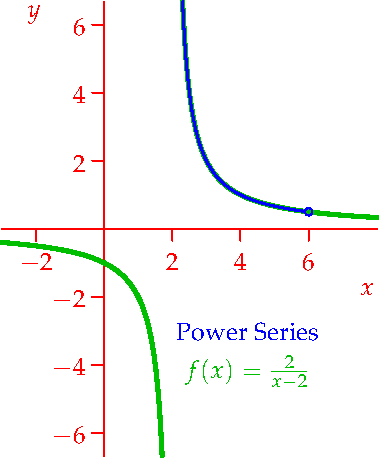
\includegraphics[scale=0.95]{powerseriesex}
	\end{minipage}
\end{example}

The example shows that we cannot blindly take limits inside an infinite sum; understanding precisely when this is possible is one of our primary goals. 


\goodbreak


\boldsubsubsection{Radius and Interval of Convergence}

The implied domain of the series in Example \ref{ex:ps1} turned out to be an \emph{interval} $(2,6)$. Somewhat amazingly, the root test (Theorem \ref{thm:roottest}) shows that the same is true for \emph{every} power series!

\begin{thm}{Root Test for Power Series}{seriesconv}
	Given a power series \smash[b]{$\sum a_n(x-c)^n$,} define\footnotemark
	\[
		R=\frac 1{\limsup\nm{a_n}^{1/n}}
	\]
	The precisely one of the following statements holds:
	\[
		\begin{array}{@{}ll}
			R\in(0,\infty)&\text{the series converges absolutely when $\nm{x-c}<R$ and diverges when $\nm{x-c}>R$}\\[5pt]
			R=\infty&\text{the series converges absolutely for all $x\in\R$}\\[5pt]
			R=0&\text{the series converges only at the center $x=c$}
		\end{array}
	\]
\end{thm}

\footnotetext{%
	Since $\nm{a_n}\ge 0$, we here adopt the conventions $\frac 10=\infty$, $\frac 1\infty=0$. With similar caveats, one can write $R=\liminf\nm{a_n}^{-1/n}$. Since every sequence has a limit superior, this really is a \emph{definition.} Whether one can easily \emph{compute} $R$ is another matter\ldots%
}

\begin{proof}
	For each fixed $x\in\R$, let $b_n=a_n(x-c)^n$ and apply the root test to $\sum b_n$, noting that
	\begin{gather*}
		\limsup\nm{b_n}^{1/n}=
		\begin{cases}
			\limsup\nm{a_n}^{1/n}\nm{x-c}=\frac 1R\nm{x-c}&\text{if $R\in(0,\infty)$}\\
			0&\text{if }R=\infty\text{ or }x=c\\
			\infty&\text{if }R=0\text{ and }x\neq c
		\end{cases}
	\end{gather*}
	In the first situation, $\limsup\nm{b_n}^{1/n}<1\iff \nm{x-c}<R$, etc.
\end{proof}

\begin{defn}{}{}
	The \emph{radius of convergence} is the value $R$ defined in Theorem \ref{thm:seriesconv}. The \emph{interval of convergence} is the set of $x\in\R$ for which the series converges; its implied domain.
	\[
		\begin{array}{c|c}
			\text{Radius of convergence}&\text{Interval of convergence}\\\hline\hline
			R\neq 0,\infty&(c-R,c+R),\ (c-R,c+R],\ [c-R,c+R)\ \text{or }[c-R,c+R]\\
			\infty&\R=(-\infty,\infty)\\
			0&\{c\}
		\end{array}
	\]
	In the first case, convergence/divergence at the endpoints of the interval of convergence must be tested for separately.
\end{defn}

The ratio test (Corollary \ref{cor:ratiotest}) provides a more user-friendly version.

\begin{cor}{Ratio Test for Power Series}{ratiops}
	If the limit exists, $R=\lim\limits_{n\to\infty}\nm{\frac{a_n}{a_{n+1}}}$.
\end{cor}

The ratio test is \emph{weaker} than the root test: as Example \ref*{ex:easyintconv}.\ref{ex:easyintconv2} shows, there exist series for which the ratio test is be inconclusive.

\goodbreak


\begin{examples}{}{easyintconv}
	\exstart The series $\sum_{n=1}^\infty \frac 1nx^n$ is centered at $0$. The ratio test tells us that
	\begin{enumerate}\setcounter{enumi}{1}
	  \begin{minipage}[t]{0.65\linewidth}\vspace{-15pt}
	  \item[]
	  \[
	  	R=\lim_{n\to\infty}\nm{\frac{a_n}{a_{n+1}}}
	  	=\lim_{n\to\infty}\frac{1/n}{1/(n+1)} 
	  	=\lim_{n\to\infty}\frac{n+1}{n}=1
	  \]
	  Test the endpoints of the interval of convergence separately:
	  \[
	  	\begin{array}{ll}
	  		x=1&\sum \frac 1n=\infty\text{ diverges}\\[5pt]
	  		x=-1&\sum \frac{(-1)^n}n\text{ converges (conditionally)}
	  	\end{array}
	  \]
	  We conclude that the interval of convergence is $[-1,1)$.\medbreak
	  It can be seen (later) that the series converges to \textcolor{Green}{$-\ln(1-x)$} on its interval of convergence. As in Example \ref{ex:ps1}, this function has a larger domain $(-\infty,-1)$, than that of the \textcolor{blue}{series}.
		\end{minipage}
		\hfill
		\begin{minipage}[t]{0.34\linewidth}\vspace{0pt}
			\flushright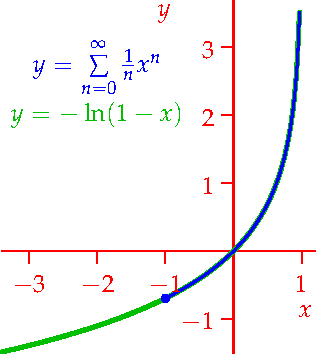
\includegraphics[scale=0.95]{powerseriesex2}
		\end{minipage}
		
		
	  \item The series $\sum_{n=1}^\infty\frac 1{n^2}x^n$ similarly has
	  \[
	  	R=\lim_{n\to\infty}\nm{\frac{a_n}{a_{n+1}}}
	  	=\lim_{n\to\infty}\frac{(n+1)^2}{n^2}=1
	  \]
		Since $\sum \frac 1{n^2}$ is absolutely convergent, we conclude that the power series also converges absolutely at $x=\pm 
		1$; the interval of convergence is $[-1,1]$.
	
		\item The series $\sum_{n=0}^\infty \frac 1{n!}x^n$ converges absolutely for all $x\in\R$, since
	  \[
	  	R=\lim_{n\to\infty}\nm{\frac{a_n}{a_{n+1}}}
	  	=\lim_{n\to\infty}\frac{(n+1)!}{n!}
	  	=\lim_{n\to\infty}(n+1)=\infty
	  \]
	  You should recall from elementary calculus that this series converges to the natural exponential function $\exp(x)=e^x$ everywhere on $\R$; indeed this is one of the common \emph{definitions} of the exponential function.
	
	
		\item The series $\sum_{n=0}^\infty n!x^n$ has $R=\lim\frac{n!}{(n+1)!}=0$. It therefore converges only at its center $x=0$.
	
	
		\item\label{ex:easyintconv2} Let $a_n=\left(\frac 23\right)^n$ if $n$ is even and $\left(\frac 32\right)^n$ if $n$ is odd. If we try to apply the ratio test to the series $\sum_{n=0}^\infty a_nx^n$, we see that
		\[
			\nm{\frac{a_n}{a_{n+1}}}=
			\begin{cases}
				\left(\frac 23\right)^{2n+1}&\text{if $n$ even}\\
				\left(\frac 32\right)^{2n+1}&\text{if $n$ odd}
			\end{cases}
			\implies \limsup\nm{\frac{a_n}{a_{n+1}}}
			=\infty\neq 0=\liminf\nm{\frac{a_n}{a_{n+1}}}
		\]
		The ratio test is therefore inconclusive. However, by the root test,
		\[
			\nm{a_n}^{1/n}=
			\begin{cases}
				\frac 23&\text{if $n$ even}\\
				\frac 32&\text{if $n$ odd}
			\end{cases}\ 
			\implies R=\frac 1{\limsup\nm{a_n}^{1/n}}=\frac 1{3/2}=\frac 23
		\]
		It is easy to check that the series diverges at $x=\pm\frac 23$; the interval of convergence is $(-\frac 23,\frac 23)$.
	\end{enumerate}
\end{examples}
\goodbreak

With the help of the root test the domain of a power series is fully understood. Limits, continuity, differentiability and integrability are more delicate. We will return to these once we've developed some of the ideas around \emph{convergence} for \emph{sequences of functions.}

\goodbreak

\begin{exercises}
	\emph{Key concepts:\quad Power Series,\quad Radius/interval of convergence $R=\frac 1{\limsup\nm{a_n}^{1/n}}$}
	
	\begin{enumerate}
		\item For each power series, find the radius and interval of convergence:
		\begin{enumerate}
		  \item \makebox[120pt][l]{$\displaystyle\sum\frac{(-1)^n}{n^24^n}x^n$\hfill(b) }\
			\makebox[140pt][l]{$\displaystyle\sum\frac{(n+1)^2}{n^3}(x-3)^n$\hfill(c) }\
			$\displaystyle\sum\sqrt nx^n$
			\item[(d)] \makebox[120pt][l]{$\displaystyle\sum\frac{1}{n^{\sqrt n}}(x+7)^n$\hfill(e) }\
			\makebox[140pt][l]{$\displaystyle\sum (x-\pi)^{n!}$\hfill(f) }\
			$\displaystyle\sum\frac{3^n}{\sqrt n}x^{2n+1}$
		\end{enumerate}
	  
	  
	  \item For each $n\in\N$ let $a_n=\left(\frac{4+2(-1)^n}{5}\right)^n$
	  \begin{enumerate}
	    \item Find $\limsup\nm{a_n}^{1/n}$, $\liminf\nm{a_n}^{1/n}$, $\limsup\nm{\frac{a_{n+1}}{a_n}}$ and $\liminf\nm{\frac{a_{n+1}}{a_n}}$.
	    \item Does the series $\sum a_n$ converge? What about $\sum (-1)^na_n$? Why?
	    \item Find the interval of convergence of the power series $\sum a_nx^n$.
	  \end{enumerate}
	  
	  
	  \item Suppose that $\sum a_nx^n$ has radius of convergence $R$. If $\limsup\nm{a_n}>0$, prove that $R\le 1$.
	  
	  
	  \item On the interval $(-\frac 23,\frac 23)$, express the series in Example \ref*{ex:easyintconv}.\ref{ex:easyintconv2} as a simple function.\par
	  (\emph{Hints: Use geometric series formulæ and the fact that the value of an absolutely convergent series is independent of rearrangements}) 
	  
	  
		\item Consider the power series
		\[
			\sum_{n=1}^\infty \frac{1}{3^nn}(x-7)^{5n+1} 
			=\frac 13(x-7)+\frac 1{18}(x-7)^6+\frac 1{81}(x-7)^{11}+\cdots 
		\]
		Since only one in five of the terms are non-zero, it is a little tricky to analyze using a naïve application of our standard tests.
		\begin{enumerate}
		  \item Explain why the ratio test for power series (Corollary \ref{cor:ratiops}) does not apply.
		  
		  \item Writing the series as $\sum a_m(x-7)^m$, observe that
		  \begin{gather*}
				a_m=\begin{cases}
				\frac 5{3^{\frac{m-1}5}(m-1)}&\text{if $m\equiv 1\mod 5$}\\
				0&\text{otherwise}
			\end{cases}%\\
			%\implies \limsup\nm{a_m}^{1/m} = \lim\frac{5^{1/m}}{3^{\frac 15-\frac 1{5m}}(m-1)^{1/m}} =3^{-1/5} \implies R=\sqrt[5]{3}
			\end{gather*}
		  Use the root test (Theorem \ref{thm:seriesconv}) and your understanding of elementary limits to directly compute the radius of convergence.
		  
		  \item Alternatively, write $\sum \frac{1}{3^nn}(x-7)^{5n+1}=\sum b_n$. Apply the ratio test for \emph{infinite} series (Corollary \ref{cor:ratiotest}): what do you observe? Use your observation to compute the radius of convergence of the original series in a simpler manner than part (a).
		  
		  \item Finally, check the endpoints to determine the interval of convergence.
		\end{enumerate}
		
		%\item Find the interval of convergence of the series $\sum 2^n(2x-1)^{2n}$
	\end{enumerate}
\end{exercises}


\clearpage


\subsection{Uniform Convergence}\label{sec:uniformconv}

In this section we consider sequences $(f_n)$ of \emph{functions} $f_n:U\to\R$ and their limits.

\begin{example}{}{seqfn}
	For each $n\in\N$, define $f_n:(0,1)\to\R:x\mapsto x^n$. Several examples are graphed.
	\begin{center}
		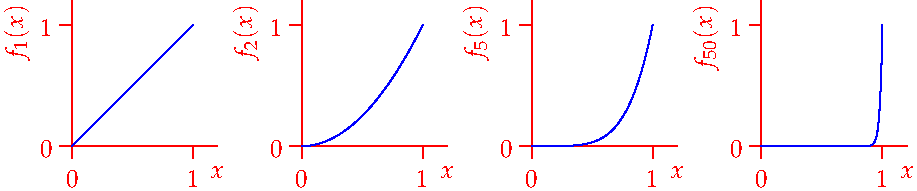
\includegraphics{seqex1}
	\end{center}
\end{example}

There are several useful notions of convergence for sequences of functions. The simplest is where, for each input $x$, $(f_n(x))$ is treated as a distinct sequence of real numbers.

\begin{defn}{}{}
	Suppose a function $f$ and a sequence of functions $(f_n)$ are given, all with domain $U$. We say that \emph{$(f_n)$ converges pointwise to $f$ on $U$} if,
	\[
		\forall x\in U,\ \lim\limits_{n\to\infty}f_n(x)=f(x)
	\]
\end{defn}

It is common to write `$f_n\to f$ pointwise.' For reference, here are two equivalent rephrasings:
\begin{enumerate}
  \item $\displaystyle \forall x\in U, \ \lim_{n\to\infty}\nm{f_n(x)-f(x)}=0$;
  \item $\textcolor{purple}{\forall x}\in U,\ \forall \epsilon>0,\ \textcolor{orange}{\exists N}$ such that $n>N\Longrightarrow \nm{f_n(x)-f(x)}<\epsilon$.
\end{enumerate}

As we'll see shortly, the relative position of the quantifiers ($\textcolor{purple}{\forall x}, \ \textcolor{orange}{\exists N}$) is crucial: in this definition, the value of $N$ is permitted to depend on $x$ as well as $\epsilon$.
\vspace*{10pt}


\begin{example*}{\ref{ex:seqfn}, mk.\ II}{}
	The sequence $(f_n)$ converges pointwise on the domain $U=(0,1)$ to\smallbreak
	\begin{minipage}[t]{0.6\linewidth}\vspace{-12pt}
	\[
		\textcolor{Green}{f:(0,1)\to\R:x\mapsto 0}
	\]
	As a sanity check, we prove this explicitly. First observe that
	\[
		\nm{f_n(x)-f(x)}=x^n
	\]
	Suppose $x\in(0,1)$, that $\epsilon>0$ is given, and let $N=\frac{\ln\epsilon}{\ln x}$. Then
	\[
		n>N\implies n\ln x<\ln\epsilon\implies x^n<\epsilon
	\]
	where the inequality switches sign since $\ln x<0$.
	\end{minipage}
	\hfill
	\begin{minipage}[t]{0.39\linewidth}\vspace{0pt}
		\flushright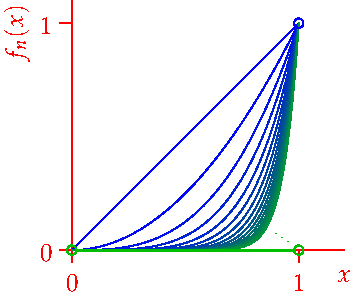
\includegraphics[scale=0.95]{seqex2}
	\end{minipage}
\end{example*}

The example is nice in that a sequence of continuous functions converges pointwise to a continuous function. Unfortunately, this desirable situation is not universal\ldots

\goodbreak

\begin{example*}[lower separated=false, sidebyside, sidebyside align=top seam, sidebyside gap=0pt, righthand width=0.39\linewidth]{\ref{ex:seqfn}, mk.\ III}{}
	Define
	\[
		g_n:(0,1]\to\R: x\mapsto x^n
	\]
	Each $g_n$ is a continuous function, however its \textcolor{Green}{pointwise limit}
	\[
		g(x)=
		\begin{cases}
			0&\text{if }x<1\\
			1&\text{if }x=1
		\end{cases}
	\]
	has a \emph{jump discontinuity} at $x=1$.
	\tcblower
	\flushright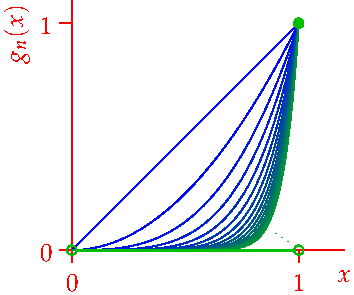
\includegraphics[scale=0.95]{seqex3}
\end{example*}

We'd like the limit of a sequence of continuous functions to itself be continuous. With this goal in mind, we make a tighter definition.


\begin{defn}[lower separated=false, sidebyside, sidebyside align=top seam, sidebyside gap=0pt, righthand width=0.32\linewidth]{}{unifconv}
	$(f_n)$ \emph{converges uniformly} to $f$ on $U$ if either
	\begin{enumerate}
	  \item $\displaystyle \sup\limits_{x\in U}\nm{f_n(x)-f(x)}\xrightarrow[n\to\infty]{}0$,\quad or,
	  \item $\forall \epsilon>0,\ \textcolor{orange}{\exists N}$ such that $\textcolor{purple}{\forall x}\in U$, $n>N\Longrightarrow \nm{f_n(x)-f(x)}<\epsilon$
	\end{enumerate}
	A common notation is $f_n\rightrightarrows f$, though we won't use it.
	\tcblower
	\flushright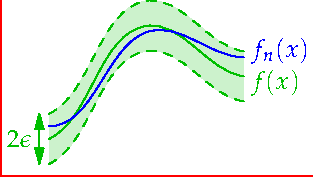
\includegraphics[scale=0.95]{unifconv1}
\end{defn}

As pictured, whenever $n>N$, the graph of $\textcolor{blue}{f_n(x)}$ must lie between $\textcolor{Green}{f(x)\pm\epsilon}$.\smallbreak

We'll show that statements 1 and 2 are equivalent momentarily. For the present, compare with the corresponding statements for pointwise convergence:
\begin{itemize}\itemsep0pt
  \item As with \emph{continuity} versus \emph{uniform continuity,} the distinction comes in the \emph{order of the quantifiers}: in uniform convergence, $x$ is quantified \emph{after} $N$ and so \emph{the same $N$ works for all locations $x$.}
  \item Uniform convergence implies pointwise convergence.
\end{itemize}


\begin{example*}{\ref{ex:seqfn}, mk.\ IV}{}
	For the final time we revisit our main example. If $f_n(x)=x^n$ and $f(x)=0$ are defined on $U=(0,1)$, then $f_n\to f$ \emph{non-uniformly.} We show this using both criteria.\medbreak
	\begin{minipage}{0.68\linewidth}\vspace{0pt}
		\begin{enumerate}
		  \item For \emph{every} $n$,
		  \[
		  	\sup_{x\in(0,1)}\nm{f_n(x)-f(x)} =\sup\{x^n:0<x<1\}=1 \not\longrightarrow 0
		  \]
		  which plainly fails to converge to zero.
		  \item Suppose the convergence were uniform and let
		  $\epsilon=\frac 12$. Then 
		  \[
		  	\exists N\in\N\text{ such that }\forall x\in (0,1),\ n>N\implies x^n<\frac 12
		  \]
		  Since $N\in\N$, a simple choice results in a contradiction;
		  \[
		  	x=\left(\frac 12\right)^{\frac 1{N+1}}\in(0,1)\implies x^{N+1}=\frac 12
		 	\]
		\end{enumerate} 
  \end{minipage}
  \hfill
  \begin{minipage}{0.31\linewidth}\vspace{0pt}
		\flushright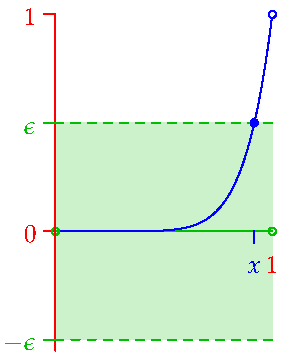
\includegraphics[scale=0.95]{unifconv2}
  \end{minipage}
\end{example*}


\goodbreak


\begin{thm}{}{}
	The criteria for uniform convergence in Definition \ref{defn:unifconv} are equivalent.
\end{thm}

\begin{proof}
	($1\Rightarrow 2$)\quad This follows immediately from the fact that
	\[
		\forall x\in U,\ \nm{f_n(x)-f(x)}\le\sup_{x\in U}\nm{f_n(x)-f(x)}
	\]
	($2\Rightarrow 1$)\quad Suppose $\epsilon>0$ is given. Then
	\[
		\exists N\in\R\text{ such that }\forall x\in U,\ n>N\implies\nm{f_n(x)-f(x)}<\frac\epsilon 2
	\]
	But then
	\[
		n>N\implies\sup_{x\in U}\nm{f_n(x)-f(x)}\le\frac\epsilon 2<\epsilon\tag*{\qedhere}
	\]
\end{proof}


Amazingly, this subtle change of definition is enough to preserve continuity.

\begin{thm}{}{unifcontlimit}
	Suppose $(f_n)$ is a sequence of continuous functions. If $f_n\to f$ uniformly, then $f$ is continuous.
\end{thm}

\begin{proof}
	We demonstrate the continuity of $f$ at $a\in U$. Let $\epsilon>0$ be given.
	\begin{itemize}
	  \item Since $f_n\to f$ uniformly,
		\[
			\exists N\text{ such that }\forall x\in U,\ n>N
			\implies\nm{f(x)-f_n(x)}<\frac\epsilon 3
		\]
		\item Choose any $n>N$. Since $f_n$ is continuous at $a$,
		\[
			\exists \delta>0\text{ such that }
			\nm{x-a}<\delta\implies\nm{f_n(x)-f_n(a)}
			<\frac\epsilon 3\tag{$\dag$}
		\]
	\end{itemize}
	Put these together with the triangle inequality to see that
	\begin{align*}
		\nm{x-a}<\delta\implies\nm{f(x)-f(a)}&\le\nm{f(x)-f_n(x)}+\nm{f_n(x)-f_n(a)}+\nm{f_n(a)-f(a)}\\
		&<\frac\epsilon 3+\frac\epsilon 3+\frac\epsilon 3=\epsilon \tag*{\qedhere}
	\end{align*}
\end{proof}

We need not have fixed $a$ at the start of the proof. Rewriting $(\dag)$ to become
\[\exists\delta>0\text{ such that }\forall x,a\in U,\ \nm{x-a}<\delta\implies\nm{f_n(x)-f_n(a)}<\frac\epsilon 3\]
proves a related result.

\begin{cor}{}{}
	Suppose $(f_n)$ is a sequence of \textbf{uniformly} continuous functions. If $f_n\to f$ uniformly, then $f$ is also \textbf{uniformly} continuous.
\end{cor}


\goodbreak


\begin{examples}{}{}
	\exstart Let $f_n(x)=x+\frac 1nx^2$. This is continuous on $\R$ for all $x$, and converges pointwise to the continuous function $f:x\mapsto x$.
	\begin{enumerate}\setcounter{enumi}{1}
	  \item[]\begin{enumerate}
	    \item On any bounded interval $[-M,M]$ the convergence $f_n\to f$ is uniform,
	    \[
	    	\sup_{x\in[-M,M]}\nm{f_n(x)-f(x)}
	    	=\sup\left\{\frac 1nx^2:x\in[-M,M]\right\}
	    	=\frac{M^2}n \xrightarrow[n\to\infty]{}0
	    \]
	    \item On any unbounded interval, $\R$ say, the convergence is non-uniform,
	    \[
	    	\sup_{x\in\R}\nm{f_n(x)-f(x)}=\sup\left\{\frac 1nx^2:x\in\R\right\}=\infty %\nxrightarrow{n\to\infty} 0
	    \]
	  \end{enumerate}
	  
	  \begin{minipage}[t]{0.53\linewidth}\vspace{0pt}
	  \item Consider $f_n(x)=\frac 1{1+x^n}$; this is continuous on $(-1,\infty)$ and converges pointwise to
	  \[
	  	\textcolor{Green}{
	  		f(x)=
		  	\begin{cases}
		  		0&\text{if }x>1\\
		  		\frac 12&\text{if }x=1\\
		  		1&\text{if }-1<x<1
		  	\end{cases}
	  	}
	  \]
	  We consider the convergence $f_n\to f$ on several intervals.
	  \end{minipage}
	  \hfill
	  \begin{minipage}[t]{0.46\linewidth}\vspace{0pt}
	  	\flushright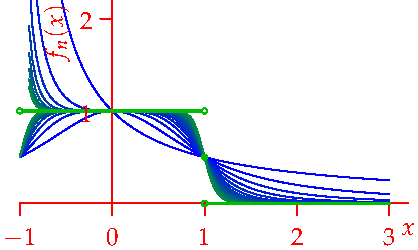
\includegraphics[scale=0.95]{seqex4}
	  \end{minipage}
	
	  \begin{enumerate}
	    \item On $[2,\infty)$, the pointwise limit is continuous. Moreover, $f_n(x)$ is decreasing, whence
	    \[
	    	\sup_{x\in[2,\infty)}\nm{f_n(x)-0}=\frac 1{1+2^n}\xrightarrow[n\to\infty]{} 0
	    \]
	    and the convergence is uniform. Alternatively; if $\epsilon\in (0,1)$, let $N=\log_2(\epsilon^{-1}-1)$, then
	    \[
	    	\forall x\ge 2,\ n>N
	    	\implies \nm{f_n(x)-0}=\frac 1{1+x^n}
	    	\le \frac 1{1+2^n}<\frac 1{1+2^N}=\epsilon
	    \]
	    The same argument shows that $f_n\to f$ uniformly on any interval $[a,\infty)$ where $a>1$.
	    \item On $[1,\infty)$ the convergence is not uniform, since the pointwise limit is discontinuous,
			\[
				f(x)=
				\begin{cases}
	    		0&\text{if }x>1\\
	    		\frac 12&\text{if }x=1
	    	\end{cases}
	    \]
	   	\item The convergence is not even uniform on the open interval $(1,\infty)$,
	    \[
	    	\sup_{x\in[1,\infty)}\nm{f_n(x)-f(x)}
	    	=\sup\left\{\frac 1{1+x^n}:x>1 \right\}
	    	=\frac 12\nxrightarrow{n\to\infty} 0
	    \]
	    \item Similarly, for any $a\in(0,1)$, the convergence $f_n\to f$ is uniform on $[0,a]$, this time to the (continuous) constant function $f(x)=1$,
	    \[
	    	\sup_{x\in[0,a]}\nm{f_n(x)-1}
	    	=\nm{1-\frac 1{1+a^n}}
	    	=\frac{a^n}{1+a^n}
	    	\xrightarrow[n\to\infty]{} 0
	    \]
	    \item Finally, on $(-1,1)$ the convergence is not uniform,
	    \[
	    	\sup_{x\in[0,1)}\nm{f_n(x)-f(x)}
	    	=\sup\left\{\frac{x^n}{1+x^n}:x\in[0,1) \right\}
	    	=\frac 12\nxrightarrow{n\to\infty} 0
	    \]
	  \end{enumerate}
	\end{enumerate}
\end{examples}


\begin{exercises}
	\emph{Key concepts:\quad Pointwise \& Uniform Convergence,\quad Uniform conv preserves continuity}
	
	\begin{enumerate}
		\item\label{exs:uniform1} For each sequence of functions defined on $[0,\infty)$:
		\begin{enumerate}
	    \item[(i)] Find the pointwise limit $f(x)$ as $n\to\infty$.
	    \item[(ii)] Determine whether $f_n\to f$ uniformly on $[0,1]$.
	    \item[(iii)] Determine whether $f_n\to f$ uniformly on $[1,\infty)$.
	  \end{enumerate}\vspace{-12pt}
	  \begin{align*}
		  \text{(a)}&\quad f_n(x)=\frac xn\qquad 
		  &\text{(b)}&\quad f_n(x)=\frac{x^n}{1+x^n}\qquad
		  &\text{(c)}&\quad f_n(x)=\frac{x^n}{n+x^n}\\[4pt]
		  \text{(d)}&\quad f_n(x)=\frac x{1+nx^2}\qquad
		  &\text{(e)}&\quad f_n(x)=\frac{nx}{1+nx^2}
	  \end{align*}
	 	
	 	
	 	\item Let $f_n(x)=\left(x-\frac 1n\right)^2$. If $f(x)=x^2$, we clearly have $f_n\to f$ pointwise on any domain.
	 	\begin{enumerate}
	 	  \item Prove that the convergence is uniform on $[-1,1]$.
	 	  \item Prove that the convergence is non-uniform on $\R$.
	 	\end{enumerate}
	  
	  
	  \item For each sequence, find the pointwise limit and decide if the convergence is uniform.
	  \begin{enumerate}
	    \item $f_n(x)=\frac{1+2\cos^2(nx)}{\sqrt n}$ for $x\in\R$.
	    \item $f_n(x)=\cos^n(x)$ on $[-\pi/2,\pi/2]$.
	  \end{enumerate}
	 	
	
		\item\label{ex:classicnonuniform} For each $n\in\N$, consider the continuous function
		\[
			f_n:[0,1]\to\R:x\mapsto nx^n(1-x)
		\]
		\begin{enumerate}
		  \item Given $0\le x<1$, let $a\in(x,1)$. Explain why
		  %Since $\lim\limits_{n\to\infty}\frac{f_{n+1}(x)}{f_n(x)}=x<a$,
		  $\exists N$ such that
		  \[
		  	n>N\implies \nm{f_{n+1}(x)}\le a\nm{f_n(x)}
		  \]
		  Hence conclude that the pointwise limit of $(f_n)$ is the zero function.
	% 	  \item For any $n,N\in\N$ prove that $n>N\implies \frac{n+1}n<\frac{N+1}N=1+\frac 1N$
	% 	  \item Suppose $x\in(0,1)$ is given and let $N\in\N$ satisfy $x<1-\frac 1N$. Prove that
	% 	  \[n>N\implies \frac{f_n(x)}{f_N(x)} =\frac{n}{n-1}\cdots\frac{N+1}Nx^{n-N}<\left(1-\frac 1{N^2}\right)^{n-N}\]
	% 	  Hence conclude that $f_n$ converges pointwise to the zero function.
		  \item Use elementary calculus $(f'_n(x)=0\Longleftrightarrow\ldots)$ to prove that the maximum value of $f_n$ is located at \textcolor{Green}{$x_n=\frac n{1+n}$}. Hence compute
			\[
				\sup_{x\in[0,1]}\nm{f_n(x)-f(x)}
			\]
			and use it to show that the convergence $f_n\to 0$ is non-uniform.
		\end{enumerate}
		\emph{This shows that the converse to Theorem \ref{thm:unifcontlimit} is false, even on a bounded interval: the continuous sequence $(f_n)$ converges \emph{non-uniformly} to a continuous function. Sketches of several $f_n$ are below.} 
		\begin{center}
			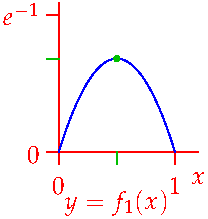
\includegraphics[scale=0.95]{seqex5}\hfill
			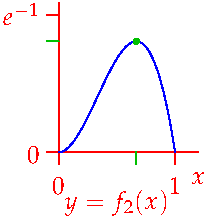
\includegraphics[scale=0.95]{seqex6}\hfill 
			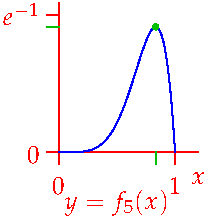
\includegraphics[scale=0.95]{seqex7}\hfill
			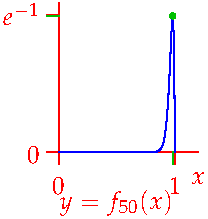
\includegraphics[scale=0.95]{seqex8}
		\end{center}
	
	
		\item Explain where the proof of Theorem \ref{thm:unifcontlimit} fails if $f_n\to f$ \emph{non-uniformly.}
	\end{enumerate}
\end{exercises}


\goodbreak


\subsection{More on Uniform Convergence}\label{sec:unifconvmore}

While we haven't yet developed calculus, our familiarity with basic differentiation and integration makes it natural to pause to consider the interaction of these concepts with sequences of functions.\smallbreak

We also consider a Cauchy-criterion for uniform convergence, which leads to the useful Weierstraß\ $M$-test.

\begin{example}{}{diffinteasy}
	Recall that $f_n(x)=x^n$ converges uniformly to $f(x)=0$ on any interval $[0,a]$ where $a<1$. We easily check that
  \[
  	\int_0^af_n(x)\,\dx
  	=\frac 1{n+1}a^{n+1}\xrightarrow[n\to\infty]{} 0 
  	=\int_0^af(x)\,\dx
  \]
  In fact the sequence of derivatives converge here also
  \[\diff xf_n(x)=nx^{n-1} \xrightarrow[n\to\infty]{} 0 =f'(x)\]
\end{example}

It is perhaps surprising that integration interacts more nicely with uniform limits than does differentiation. We therefore consider integration first.

\begin{thm}{}{unifintegral}
	Let $f_n\to f$ uniformly on $[a,b]$ where the functions $f_n$ are integrable. Then $f$ is integrable on $[a,b]$ and
	\[
		\lim_{n\to\infty}\int_a^bf_n(x)\dx=\int_a^bf(x)\dx
	\]
\end{thm}

\begin{proof}
	Given $\epsilon>0$, note that $\int_a^b\frac\epsilon{2(b-a)}\,\dx=\frac\epsilon 2$. Since $f_n\to f$ uniformly, $\exists N$ such that\footnotemark
	\begin{align*}
		\forall x\in [a,b],\ n>N
		&\implies \nm{f_n(x)-f(x)}<\frac\epsilon{2(b-a)}\\
		&\implies f_n(x)-\frac\epsilon{2(b-a)}<f(x)< f_n(x)+\frac\epsilon{2(b-a)}\\
		&\implies \int_a^b f_n(x)\,\dx-\frac\epsilon 2\le \int_a^bf(x)\,\dx
		\le \int_a^b f_n(x)\,\dx+\frac\epsilon 2\\
		&\implies \nm{\int_a^bf_n(x)\,\dx-\int_a^bf(x)\,\dx}
		\le \frac\epsilon 2<\epsilon\tag*{\qedhere}
	\end{align*}
\end{proof}

\footnotetext{%
	This assumes $f$ is already integrable. Once we've properly defined (Riemann/Darboux) integrability at the end of the course, we can insert the following
	\[
		\int_a^b f_n(x)\,\dx-\frac\epsilon 2\le L(f)
		\le U(f)\le \int_a^b f_n(x)\,\dx+\frac\epsilon 2
		\implies 0\le U(f)-L(f)\le \epsilon\implies U(f)=L(f)
	\]
	where $U(f)$ and $L(f)$ are the upper and lower Darboux integrals of $f$; equality shows that $f$ is integrable on $[a,b]$.%
}

The appearance of uniform convergence in the proof is subtle. If $N=N(\epsilon)$ were allowed to depend on $x$, then the integral $\int_a^bf_n(x)\,\dx$ would be meaningless: Which $n$ would we consider? Larger than $N(x,\epsilon)$ for \emph{which} $x$? Taking $n$ `larger' than \emph{all} the $N(x,\epsilon)$ might produce the absurdity $n=\infty$!

\goodbreak

\begin{examples}{}{intnotconvout}
	\exstart Uniform convergence is not required for the integrals to converge as we'd like. For instance, recall that extending the previous example to the domain $[0,1]$ results in non-uniform convergence; however, we still have
	\[
		\int_0^1f_n(x)\,\dx=\frac 1{n+1}\xrightarrow[n\to\infty]{} 0 =\int_0^1f(x)\,\dx
	\]
  %Since $f$ is discontinuous, the final integral requires a little care.
  
	\begin{enumerate}\setcounter{enumi}{1}
	  \item\label{ex:intnotconv} To obtain a sequence of functions $f_n\to f$ for which $\int f_n\nrightarrow\int f$ requires a bit of creativity. Consider the sequence\smallbreak
	  \begin{minipage}[t]{0.6\linewidth}\vspace{-15pt}
		  \begin{align*}
			  f_n&:[-1,1]\to\R :x\mapsto 
			  \begin{cases}
			  	n-n^2x&\text{if }0<x<\frac 1n\\
			  	0&\text{otherwise}
			  \end{cases}
		  \end{align*}
		  If $0<x<1$, then for large $n\in\N$ we have
		  \[
		  	x\ge\frac 1n\implies f_n(x)=0
		  \]
	  \end{minipage}
	  \hfill
	  \begin{minipage}[t]{0.39\linewidth}\vspace{-10pt}
	  \flushright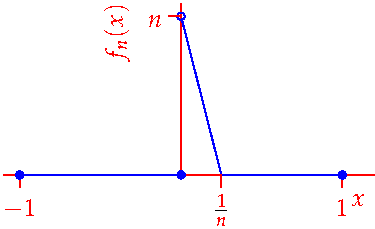
\includegraphics[scale=0.95]{seqex10}
	  \end{minipage}\par
	  We conclude that $f_n\to 0$ pointwise. Since the area under $f_n$ is a triangle with base $\frac 1n$ and height $n$, the integral is constant and \emph{non-zero};
	  \[
	  	\int_{-1}^1 f_n(x)\,\dx=\frac 12\neq 0=\int_{-1}^1f(x)\,\dx
	  \]
	  It should be obvious that the convergence $f_n\to 0$ is non-uniform; why?
	\end{enumerate}
\end{examples}


\boldinline{Derivatives and Uniform Limits}

We've already seen that a uniform limit of differentiable functions \emph{might} be differentiable (Example \ref{ex:diffinteasy}). As the next example shows, this should not be expected in general, since even uniform limits of differentiable functions can have corners.

\begin{example}[lower separated=false, sidebyside, sidebyside align=top seam, sidebyside gap=0pt, righthand width=0.4\linewidth]{}{}
	For each $n\in\N$, consider the function
	\[
		f_n:\R\to\R:x\mapsto 
		\begin{cases}
			\nm x&\text{if }\nm x\ge\frac 1n\\
			\frac n2x^2+\frac 1{2n}&\text{if }\nm x<\frac 1n
		\end{cases}
	\]
	\begin{itemize}
	 	\item Each $f_n$ is differentiable: $f'_n(x)=
	 	\begin{cases}
		  1&\text{if }x\ge\frac 1n\\
		  nx&\text{if }\nm x<\frac 1n\\
		  -1&\text{if }x\le -\frac 1n
	  \end{cases}$
	  \item $f_n$ converges pointwise to \textcolor{Green}{$f(x)=\nm x$}, which is \emph{non-differentiable} at $x=0$.
	  \item $f_n\to f$ uniformly since
	  \[
	  	\sup_{x\in[-1,1]}\nm{f_n(x)-f(x)} =f_n(0)=\frac 1{2n}\to 0
	  \]
	\end{itemize}
	\tcblower
	\flushright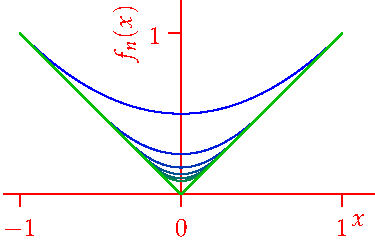
\includegraphics[scale=0.95]{seqex9}\\
	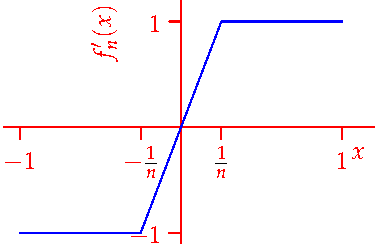
\includegraphics[scale=0.95]{seqex9-1}
\end{example}

\goodbreak


If our goal is to transfer differentiability to the limit of a sequence of functions, then we have some work to do.

\begin{thm}{}{unifderiv}
	Suppose $(f_n)$ is a sequence and $f,g$ functions, all with domain $[a,b]$. Suppose also:
	\begin{itemize}
	  \item $f_n\to f$ pointwise;
	  \item Each $f_n$ is differentiable with continuous derivative;\footnotemark
	  \item $f_n'\to g$ uniformly.
	\end{itemize}
	Then $f_n\to f$ uniformly on $[a,b]$ and $f$ is differentiable with derivative $g$.
\end{thm}

\footnotetext{%
	Without this continuity assumption, the fundamental theorem of calculus doesn't apply and the proof requires an alternative approach. One can also weaken the hypotheses: if $f'_n\to g$ uniformly and $(f_n(x))$ converges for \emph{at least one} $x\in [a,b]$, then there exists $f$ such that $f_n\to f$ is uniform and $f'=g$.%
}

The issue in the previous example is that the \emph{pointwise limit} of the derived sequence $(f'_n)$ is discontinuous at $x=0$ and therefore $f'_n\to g$ isn't uniform! 

\begin{proof}
	For any $x\in [a,b]$, the fundamental theorem of calculus (part II) tells us that
	\[
		\int_a^x f'_n(t)\,\dt  = f_n(x)-f_n(a)
	\]
	As $n\to\infty$, Theorem \ref{thm:unifintegral} says the left side converges to $\int_a^x g(t)\,\dt$ and the right to $f(x)-f(a)$ (both pointwise). Since $f_n'\to g$ uniformly, we see that $g$ is continuous and can apply the fundamental theorem (part I): $\int_a^xg(t)\,\dt=f(x)-f(a)$ is differentiable with derivative $g$.\smallbreak
	The uniformity of the convergence $f_n\to f$ follows from Exercise \ref{ex:derivunifconvtidy}.
\end{proof}


\boldsubsubsection{Uniformly Cauchy Sequences and the Weierstraß $M$-Test}

Recall that one may use Cauchy sequences to demonstrate convergence \emph{without knowing the limit in advance.} An analogous discussion is available for sequences of functions.


\begin{defn}{}{}
	A sequence of functions $(f_n)$ is \emph{uniformly Cauchy} on $U$ if
	\[
		\forall\epsilon>0,\ \exists N\in\N \text{ such that }\forall x\in U,\ m,n>N\implies\nm{f_n(x)-f_m(x)}<\epsilon
	\]
\end{defn}

\begin{example}{}{unifcauchy}
	Let $f_n(x)=\sum\limits_{k=1}^n\frac 1{k^2}\sin k^2x$ be defined on $\R$. Given $\epsilon>0$, let $N=\frac 1\epsilon$, then\vspace{-10pt}
	\begin{align*}
		m>n>N\implies \nm{f_m(x)-f_n(x)}
		&=\nm{\sum_{k=n+1}^m\frac 1{k^2}\sin k^2x} 
		\le\sum_{k=n+1}^m\frac 1{k^2} \le\sum_{k=n+1}^m\frac 1{k(k-1)}\\
		&=\sum_{k=n+1}^m\frac 1{k-1}-\frac 1k 
		=\frac 1n-\frac 1m<\frac 1N=\epsilon
	\end{align*}
	whence $(f_n)$ is uniformly Cauchy.
\end{example}


\goodbreak


As with sequences of real numbers, uniformly Cauchy sequences converge; in fact uniformly!

\begin{thm}{}{}
	A sequence $(f_n)$ is uniformly Cauchy on $U$ if and only if it converges uniformly to some $f:U\to\R$.
\end{thm}

\begin{proof}
	\begin{description}
		\item[$(\Rightarrow)$] Let $(f_n)$ be uniformly Cauchy on $U$. For each $x\in U$, the sequence $(f_n(x))\subseteq\R$ is Cauchy and thus convergent. Define $f:U\to\R$ to be the pointwise limit:
		\[
			f(x):=\lim\limits_{n\to\infty}f_n(x)
		\]
		We claim that $f_n\to f$ uniformly. Let $\epsilon>0$ be given, then $\exists N\in\N$ such that
		\begin{align*}
			m>n>N&\implies \nm{f_n(x)-f_m(x)}<\frac\epsilon 2\\
			&\implies f_n(x)-\frac\epsilon 2<f_m(x)<f_n(x)+\frac\epsilon 2\\
			&\implies f_n(x)-\frac\epsilon 2\le f(x)\le f_n(x)+\frac\epsilon 2 \tag{take limits as $m\to\infty$}\\
			&\implies \nm{f_n(x)-f(x)}\le\frac\epsilon 2<\epsilon
		\end{align*}
		\item[$(\Leftarrow)$] This is Exercise \ref{ex:cauchyexproof}.\qedhere
	\end{description}
\end{proof}


\begin{example*}{\ref{ex:unifcauchy}, mk.\ II}{}
	Since $(f_n)$ is uniformly Cauchy on $\R$, it converges uniformly to some $f:\R\to\R$. It seems reasonable to write
	\[
		f(x)=\sum\limits_{n=1}^\infty\frac 1{n^2}\sin n^2x
	\]
	The graph of this function looks somewhat bizarre:
	\begin{center}
		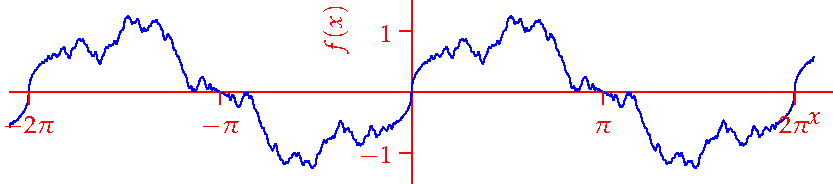
\includegraphics[scale=0.95]{unifcauchy}
	\end{center}
	Since each $f_n$ is (uniformly) continuous, Theorem \ref{thm:unifcontlimit} says that $f$ is also (uniformly) continuous. By Theorem \ref{thm:unifintegral}, $f(x)$ is integrable, indeed
	\[
		\int_a^bf(x)\,\dx
		=\lim_{n\to\infty}\sum_{k=1}^n -k^{-4}\cos k^2x\big|_a^b 
		=\sum_{n=1}^\infty \frac 1{n^4}(\cos n^2a-\cos n^2b)
	\]
	which converges (comparison test) for all $a,b$. By contrast, the derived sequence 
	\[
		f'_n(x)=\sum\limits_{k=1}^n \cos k^2x
	\]
	does not converge for \emph{any} $x$ since $\lim\limits_{n\to\infty}\cos n^2x\neq 0$. We should therefore expect (though we offer no proof) that $f$ is nowhere differentiable.
\end{example*}


\goodbreak


The example generalizes. Suppose $(g_k)$ is a sequence of functions on $U$ and define the \emph{series} $\sum g_k(x)$ as the pointwise limit of the sequence $(f_n)$ of partial sums
\[
	\sum_{k=k_0}^\infty g_k(x):=\lim\limits_{n\to\infty}f_n(x)
	\quad\text{where}\quad 
	f_n(x)=\sum_{k=k_0}^ng_k(x)
\]
whenever the limit exists. The series is said to converge uniformly whenever $(f_n)$ does so. Theorems \ref{thm:unifcontlimit}, \ref{thm:unifintegral} and \ref{thm:unifderiv} immediately translate.

\begin{cor}{}{unifseries}
	Let $\sum g_k$ be a series of functions converging uniformly on $U$. Then:
	\begin{enumerate}
	  \item If each $g_k$ is (uniformly) continuous then $\sum g_k$ is (uniformly) continuous.
	  \item If each $g_k$ is integrable, then $\int\sum g_k(x)\,\dx=\sum\int g_k(x)\,\dx$.
	  \item If each $g_k$ is continuously differentiable, and the sequence of derived partial sums $f'_n$ converges uniformly, then $\sum g_k$ is differentiable and $\diff x\sum g_k(x)=\sum g'_k(x)$.
	\end{enumerate}
\end{cor}

As an application of the uniform Cauchy criterion, we obtain an easy test for uniform convergence.

\begin{thm}{Weierstraß $M$-test}{mtest}
	Suppose $(g_k)$ is a sequence of functions on $U$. Moreover assume:
	\begin{enumerate}
	  \item $(M_k)$ is a non-negative sequence such that $\sum M_k$ converges.
	  \item Each $g_k$ is bounded by $M_k$; that is $\nm{g_k(x)}\le M_k$.
	\end{enumerate}
	Then $\sum g_k(x)$ converges uniformly on $U$.
\end{thm}

\begin{proof}
	Let $f_n(x)=\sum\limits_{k=k_0}^ng_k(x)$ define the sequence of partial sums. Since $\sum M_k$ converges, its sequence of partial sums is Cauchy (the \emph{Cauchy criterion} for infinite series); given $\epsilon>0$,
	\[
		\exists N\text{ such that }m>n>N
		\implies \sum_{k=n+1}^m M_k<\epsilon
	\]
	However, by assumption,
	\[
		m>n>N\implies \nm{f_m(x)-f_n(x)}
		=\nm{\sum_{k=n+1}^mg_k(x)} 
		\le \sum_{k=n+1}^m\nm{g_k(x)} 
		\le\sum_{k=n+1}^mM_k<\epsilon
	\]
	The sequence of partial sums is uniformly Cauchy and thus uniformly convergent.
\end{proof}

\begin{example}{}{mtestex}
	Given the series $\sum\limits_{n=1}^\infty\frac{1+\cos^2(nx)}{n^2}\sin(nx)$, we clearly have
	\[
		\nm{\frac{1+\cos^2(nx)}{n^2}\sin(nx)}
		\le\frac 2{n^2}\text{ for all }x\in\R
	\]
	Since $\sum\frac 2{n^2}$ converges, the $M$-test shows that the original series converges uniformly on $\R$.
\end{example}

\goodbreak

\begin{exercises}
	\emph{Key concepts:\quad Uniform convergence preseves integration,\quad Uniform Cauchyness,\quad $M$-test}

	\begin{enumerate}
		\item For each $n\in\N$, let $f_n(x)=nx^n$ when $x\in[0,1)$ and $f_n(1)=0$.
		\begin{enumerate}
	    \item Prove that $f_n\to 0$ pointwise on $[0,1]$.\par
	    (\emph{Hint: recall Exercise \ref*{sec:uniformconv}.\ref{ex:classicnonuniform} if you're not sure how to prove this})
	    \item By considering the integrals $\int_0^1f_n(x)\,\dx$ show that $f_n\to 0$ is not uniform.
	  \end{enumerate}
	  
	  
	  \item\label{ex:cauchyexproof} Prove that if $f_n\to f$ uniformly, then the sequence $(f_n)$ is uniformly Cauchy.
	  
	  
	  \item\begin{enumerate}
	    \item Suppose $(f_n)$ is a sequence of bounded functions on $U$ and suppose that $f_n\to f$ converges uniformly on $U$. Prove that $f$ is bounded on $U$.
	    \item Give an example of a sequence of bounded functions $(f_n)$ converging pointwise to $f$ on $[0,\infty)$, but for which $f$ is \emph{unbounded.}
	  \end{enumerate}
	  
	  
	  \item The sequence defined by $f_n(x)=\frac{nx}{1+nx^2}$ (Exercise \ref{sec:uniformconv}.1) converges uniformly on any closed interval $[a,b]$ where $0<a<b$.
	  \begin{enumerate}
	    \item Check explicitly that $\int_a^b f_n(x)\,\dx\to \int_a^bf(x)\,\dx$, where $f=\lim f_n$.
	    \item Is the same thing true for derivatives?
	  \end{enumerate}
	  
	 	\item Let $f_n(x)=n^{-1}\sin n^2x$ be defined on $\R$.
	 	\begin{enumerate}
	 	  \item Prove that $f_n$ converges uniformly on $\R$.
	 	  \item Check that $\int_0^x f_n(t)\,\dt$ converges for any $x\in\R$.
	 	  \item Does the derived sequence $(f_n')$ converge? Explain.
	 	\end{enumerate}
	  
	  
	%   \item As another example, we've already seen (page \pageref{ex:classicnonuniform}) that the pointwise convergence $f_n\to 0$ where $f_n(x)=nx^n(1-x)$ is not uniform. However the integrals still converge;
	% 	\[\int_0^1f_n(x)\,\dx=\frac n{n+1}-\frac n{n+2}\xrightarrow[n\to\infty]{} 0=\int_0^1f(x)\,\dx\]
		

		\item Use the $M$-test to prove that $\smash[b]{\sum\limits_{n=1}^\infty\frac{x^n}{n^2}}$ defines a continuous function on $[-1,1]$.
	  
	  
		\item Prove that $\sum\limits_{n=1}^\infty\frac{x^n\sin x}{(n+1)^32^n}$ converges uniformly to a continuous function on the interval $[-2,2]$.
	
	
		\item Prove that if $\sum g_k$ converges uniformly on a set $U$ and if $h$ is a bounded function on $U$, then $\sum hg_k$ converges uniformly on $U$.\par
	 	(\emph{Warning: you cannot simply write $\sum hg_k=h\sum g_k$})
	
	
	% 	\item $f_n(x)=n^{-1}e^{-nx}$ on $[0,\infty)$ converges uniformly to $f(x)=0$ since $\nm{f_n(x)}\le \frac 1n$. However
	% \[f'_n(x)=-e^{-nx}\]
	% only converges to $f'(x)=0$ when $x>0$, and only uniformly so on intervals $[a,\infty)$ where $a>0$.\goodbreak	
	
	
		\item Consider Example \ref*{ex:intnotconvout}.\ref{ex:intnotconv}.
		\begin{enumerate}
		  \item Check explicitly that the convergence isn't uniform by computing $\sup\limits_{x\in[-1,1]}\nm{f_n(x)-f(x)}$
		  \item Prove that $f_n\to 0$ pointwise on $(0,1]$ using the $\epsilon$--$N$ definition of convergence: that is, given $\epsilon>0$ and $x\in(0,1]$, find an explicit $N(x,\epsilon)$ such that
	  	\[
	  		n>N\implies \nm{f(x)}<\epsilon
	  	\]
	  	What happens to your choice of $N(x,\epsilon)$ as $x\to 0^+$?
		\end{enumerate}
		
		
		\item\label{ex:derivunifconvtidy} Suppose $(f_n')$ converges uniformly on $[a,b]$ and that each $f_n'$ is continuous.
		\begin{enumerate}
		  \item Use the fact that $(f_n')$ is uniformly Cauchy to prove that $(f_n)$ is uniformly Cauchy and thus converges uniformly to some function $f$.\par
			(\emph{Hint: $\nm{f_n(x)-f_m(x)}=\nm{\int_a^xf_n'(t)-f_m'(t)\,\dt}\ldots$})
			\item Explain why we need not have assumed the existence of $f$ in Theorem \ref{thm:unifderiv}.
		\end{enumerate}
	\end{enumerate}
\end{exercises}


\goodbreak



\subsection{Differentiation and Integration of Power Series}\label{sec:diffintpower}

We now specialize our recent results to power series. While everything will be stated for series centered at $x=0$, all are easily translated to arbitrary centers.

\begin{thm}{}{unifpowerseries}
	Let $\sum a_nx^n$ be a power series with radius of convergence $R>0$ and let $T\in(0,R)$. Then:
	\begin{enumerate}
	  \item The series converges uniformly on $[-T,T]$.
	  \item The series is uniformly continuous on $[-T,T]$ and continuous on $(-R,R)$.
	\end{enumerate} 
\end{thm}

%\vfil

\begin{proof}
	This is a straightforward application of the Weierstraß $M$-test (Theorem \ref{thm:mtest}). For each $k$, define $M_k=\nm{a_k}T^k$, and observe that
	\[
		T<R\implies \sum a_nT^n\text{ converges absolutely }\implies \sum M_k\text{ converges}
	\]
	By the $M$-test and Corollary \ref{cor:unifseries}, the power series converges uniformly on $[-T,T]$ to a uniformly continuous function.
	\medbreak
	Finally, every $x\in(-R,R)$ lies in some such interval (take $T=\nm x$), whence the power series is continuous on $(-R,R)$.
\end{proof}

\begin{example}{}{geometricps}
	On its interval of convergence $(-1,1)$, the geometric series \smash[b]{$\sum\limits_{n=0}^\infty x^n$} converges pointwise to $\frac 1{1-x}$; convergence is uniform on any interval $[-T,T]\subseteq(-1,1)$.
	\smallbreak
	We needn't use the Theorem for this is simple to verify directly: writing $f,f_n$ for the series and its partial sums,
	\begin{gather*}
		\nm{f_n(x)-f(x)}=\nm{\frac{1-x^{n+1}}{1-x}-\frac 1{1-x}}
		=\nm{\frac{x^{n+1}}{1-x}}\\
		\implies \sup_{x\in [-T,T]}\nm{f_n(x)-f(x)}
		=\frac{T^{n+1}}{1-T} \xrightarrow[n\to\infty]{} 0
	\end{gather*}
	\smallbreak
	By contrast, the convergence is non-uniform on $(-1,1)$, since
	\[
		\sup_{x\in(-1,1)}\nm{f_n(x)-f(x)}=\infty
	\]
\end{example}


\begin{thm}{}{psintdiff}
	Suppose a power series $\sum a_nx^n$ has radius of convergence $R>0$. Then the series is integrable and differentiable term-by-term on the interval $(-R,R)$. Indeed for any $x\in(-R,R)$,
	\[
		\diff x\sum\limits_{n=0}^\infty a_nx^n
		=\sum\limits_{n=1}^\infty na_nx^{n-1}
		\quad\text{and}\quad
		\int_0^x\sum\limits_{n=0}^\infty a_nt^n\,\dt
		=\sum\limits_{n=0}^\infty \frac{a_n}{n+1}x^{n+1}
	\]
	where both series also have radius of convergence $R$.
\end{thm}


\goodbreak


\begin{proof}
	Let $f(x)=\sum a_nx^n$ have radius of convergence $R$, and observe that
	\[
		\limsup\nm{na_n}^{1/n}
		=\lim n^{1/n}\limsup\nm{a_n}^{1/n}=\frac 1R
	\]
	whence $\sum na_nx^n$ also has radius of convergence $R$. At any given non-zero $x\in(-R,R)$, we may write
	\[
		\textcolor{blue}{\sum\limits_{n=1}^\infty na_nx^{n-1}}
		=x^{-1}\sum\limits_{n=1}^\infty na_nx^n
	\]
	to see that the \textcolor{blue}{derived series} also has radius of convergence $R$. On any interval $[-T,T]\subseteq (-R,R)$, the derived series converges uniformly (Theorem \ref{thm:unifpowerseries}). Since each $a_nx^n$ is continuously differentiable, Corollary \ref{cor:unifseries} says that $f$ is differentiable on $[-T,T]$ and that
	\[
		f'(x)=\sum\limits_{n=0}^\infty\diff xa_nx^n
		=\sum\limits_{n=1}^\infty na_nx^{n-1}
	\]
	Since any $x\in(-R,R)$ lies in some such interval $[-T,T]$, we are done.
	\medbreak
	Exercise \ref{ex:psintegralproof} discusses the corresponding result for integration.
\end{proof}


We postpone the canonical examples until after the next result.


\boldsubsubsection{Continuity at Endpoints?}

There is one small hole in our analysis. A series $\sum a_nx^n$ with radius of convergence $R$ converges and is continuous on $(-R,R)$. But what if it also converges at $x=\pm R$? Is the series continuous at the endpoints? The answer is yes, though demonstrating this small benefit requires a lot of work!

\begin{thm}{Abel's Theorem}{}
	Power series are continuous on their full interval of convergence.
\end{thm}


\begin{examples}{}{abel}
	\exstart\phantomsection\label{ex:abel1} Apply our results to the geometric series;
	\begin{gather*}
		\frac 1{(1-x)^2}=\diff x\frac 1{1-x}=\sum_{n=1}^\infty nx^{n-1}=\sum_{n=0}^\infty (n+1)x^n=1+2x+3x^2+4x^3+\cdots\\
		\ln(1-x)=-\int_0^x\frac 1{1-t}\,\dt= -\sum_{n=0}^\infty\frac 1{n+1}x^{n+1}
	  =-\sum_{n=1}^\infty \frac 1nx^n=-\left(x+\frac 12x^2+\frac 13x^3+\cdots\right)
	\end{gather*}
	where both are valid on $(-1,1)$. In fact the first series has exactly this interval of convergence, whereas the second has $[-1,1)$. By Abel's Theorem and the fact that logarithms are continuous, we have equality at $x=-1$ and recover the famous identity
	\[
		\ln 2=\sum_{n=1}^\infty \frac{(-1)^{n+1}}{n}=1-\frac 12+\frac 13-\frac 14+\cdots
	\]
	This also shows that while integrated and differentiated series have the same radius of convergence as the original, convergence at the endpoints need not be the same.
		
	\begin{enumerate}\setcounter{enumi}{1}  
		\item Substitute $x\mapsto -x^2$ in the geometric series and integrate term-by-term: if $\nm x<1$, then
		\[
			\frac 1{1+x^2}=\sum_{n=0}^\infty(-1)^nx^{2n} 
			\implies  \arctan x=\sum_{n=0}^\infty\frac{(-1)^n}{2n+1}x^{2n+1}
		\]
		In fact the arctangent series also converges at $x=\pm 1$; Abel's Theorem says it is continuous on $[-1,1]$. Since arctangent is continuous (on $\R$!) we recover another famous identity
		\[
			\frac\pi 4=\arctan 1
			=\sum_{n=0}^\infty\frac{(-1)^n}{2n+1}
			=1-\frac 13+\frac 15-\frac 17+\cdots
		\]
		As with the identity for $\ln 2$, this is a very slowly converging alternating series and therefore doesn't provide an efficient method for approximating $\pi$.
	  
	  \item\label{ex:abel3} The series $\displaystyle f(x)=\sum_{n=0}^\infty \frac{(-1)^n}{(2n)!}x^{2n}$ has radius of convergence $\infty$. Differentiate to obtain
		\[
			f'(x)=\sum_{n=1}^\infty \frac{(-1)^nx^{2n-1}}{(2n-1)!}
			=\sum_{n=0}^\infty \frac{(-1)^{n+1}}{(2n+1)!}x^{2n+1}
		\]
		This series is also valid for all $x\in\R$. Differentiating again,
		\[
			f''(x)=\sum_{n=0}^\infty \frac{(-1)^{n+1}}{(2n)!}x^{2n}
			=-\sum_{n=0}^\infty \frac{(-1)^n}{(2n)!}x^{2n}=-f(x)
		\]
		Recalling that $f(x)=\cos x$ is the unique solution to the initial value problem
		\[
			\begin{cases}
				f''(x)=-f(x)\\
				f(0)=1,\ f'(0)=0
			\end{cases}
		\]
		We conclude that, $\forall x\in\R$,
		\[
			\cos x=\sum_{n=0}^\infty \frac{(-1)^n}{(2n)!}x^{2n} 
			\qquad 
			\sin x=-f'(x)=\sum_{n=0}^\infty \frac{(-1)^n}{(2n+1)!}x^{2n+1}
		\]
	\end{enumerate}
\end{examples}

\phantomsection\label{pg:expseriesdefn}
These last expressions can be taken as the \emph{definitions} of sine and cosine. As promised earlier, continuity and differentiability of these functions now come for free! The only real downside of this definition is believing that it has anything to do with right-triangles!\smallbreak
We can similarly define other common transcendental functions using power series: for instance
\[
	\exp(x)=\sum\limits_{n=0}^\infty \frac 1{n!}x^n %,\qquad \cosh x=\frac{e^x+e^{-x}}2=\sum_{n=0}^\infty \frac{x^{2n}}{(2n)!},\qquad \sinh x=\frac{e^x-e^{-x}}2=\sum_{n=0}^\infty \frac{x^{2n+1}}{(2n+1)!}
\]
Example \ref{ex:abel}.1 could also be taken as a definition of the logarithm on the interval $(0,2]$, 
\[
	\ln x=\ln(1-(1-x))=-\sum_{n=1}^\infty \frac 1n(1-x)^n 
	=\sum_{n=1}^\infty \frac{(-1)^{n+1}}n(x-1)^n
\]
though this is unnecessary since it is more natural to define $\ln$ as the inverse of the exponential.


\goodbreak


\boldsubsubsection{Proof of Abel's Theorem (non-examinable)}

This requires a lot of work, so feel free to omit on a first reading!\bigbreak

First observe that there is nothing to check unless $0<R<\infty$. By the change of variable $x\mapsto \pm\frac xR$, it is enough for us to prove the following:
\[
	\sum\limits_{n=0}^\infty a_n\text{ convergent and } 
	f(x)=\sum\limits_{n=0}^\infty a_nx^n\text{ on }(-1,1)
	\implies\lim\limits_{x\to 1^-}f(x)=\sum\limits_{n=0}^\infty a_n
\]

\begin{proof}
	Let \smash[b]{$s_n=\sum\limits_{k=0}^n a_k$} and write $s=\lim s_n=\sum a_n$. It is an easy exercise to check that
	\[
		\sum_{k=0}^na_kx^k =s_nx^n+(1-x)\sum_{k=0}^{n-1}s_kx^k
	\]
	% , by convention $s_{-1}:=0$ and denote $s=\sum_{n=0}^\infty a_n$. For any $x\in(-1,1)$, observe that
	% \begin{align*}
	% \sum_{k=0}^na_kx^k =&\sum_{k=0}^n(s_k-s_{k-1})x^k =\sum_{k=0}^ns_kx^k-\sum_{k=0}^{n-1}s_kx^{k+1}=s_nx^n+(1-x)\sum_{k=0}^{n-1}s_kx^k
	% \end{align*}
	If $\nm x<1$, then (since $s_n\to s$) $\lim s_nx^n=0$, whence we obtain
	\[
		\forall x\in(-1,1),\ f(x)=(1-x)\sum_{n=0}^{\infty}s_nx^n
	\]
	Let $\epsilon\in(0,1)$ be given and fix $x\in(0,1)$. Then
	\[
		\exists N\in\N\text{ such that }n>N\implies \nm{s_n-s}<\frac\epsilon 2 \tag{$\ast$}
	\]
	Use the geometric series formula $\sum\limits_{n=0}^{\infty}x^n=\frac 1{1-x}$ and write $h(x)=(1-x)\nm{\sum\limits_{n=0}^N(s_n-s)x^n}$ to observe
	\begin{align*}
		\nm{f(x)-s}
		&=\nm{(1-x)\sum_{n=0}^{\infty}s_nx^n-s} 
		=\nm{(1-x)\sum_{n=0}^{\infty}s_nx^n-s(1-x)\sum_{n=0}^{\infty}x^n}\\
		&=\nm{(1-x)\sum_{n=0}^{\infty}(s_n-s)x^n} 
		=(1-x)\nm{\sum_{n=0}^N(s_n-s)x^n+\sum_{n=N+1}^\infty(s_n-s)x^n}\\
		&\le (1-x)\nm{\sum_{n=0}^N(s_n-s)x^n}+(1-x)\nm{\sum_{n=N+1}^\infty(s_n-s)x^n} \tag{$\triangle$-inequality}\\
		&<h(x)+\frac\epsilon 2(1-x)\nm{\sum_{n=N+1}^\infty x^n} \tag{by ($\ast$)}\\
		&\le h(x)+\frac\epsilon 2
	\end{align*}
	Since $h>0$ is continuous and $h(1)=0$, $\exists \delta>0$ such that $x\in(1-\delta,1)\Longrightarrow h(x)<\frac\epsilon 2$ (the computation of a suitable $\delta$ is another exercise).\medbreak
	We conclude that $\lim\limits_{x\to 1^-}f(x)=s$.
	%  and define $S=\max\{\nm{s_n-s}:n\le N\}$ to observe
	% \begin{align*}
	% \nm{f(x)-s}&=\nm{(1-x)\sum_{n=0}^{\infty}s_nx^n-s} =\nm{(1-x)\sum_{n=0}^{\infty}s_nx^n-s(1-x)\sum_{n=0}^{\infty}x^n}\\
	% &=\nm{(1-x)\sum_{n=0}^{\infty}(s_n-s)x^n} =(1-x)\nm{\sum_{n=0}^N(s_n-s)x^n+\sum_{n=N+1}^\infty(s_n-s)x^n}\\
	% &\le(1-x)\sum_{n=0}^N S x^n+ (1-x)\nm{\sum_{n=N+1}^\infty(s_n-s)x^n}\\
	% &\le S(1-x)\frac{1-x^{N+1}}{1-x}+ \frac\epsilon 2(1-x)\nm{\sum_{n=N+1}^\infty x^n}\\
	% &=S(1-x^{N+1})+ \frac\epsilon 2
	% \end{align*}
	% To finish the proof, let $\delta=1-\left(1-\frac\epsilon{2S}\right)^{\frac 1{N+1}}$ to observe that
	% \[x\in(1-\delta,1)\implies x>\left(1-\frac\epsilon{2S}\right)^{\frac 1{N+1}}\implies S(1- x^{N+1})<\frac\epsilon 2\tag*{\qedhere}\]
\end{proof}

\clearpage

\begin{exercises}
	\emph{Key concepts:\quad Power series continuous on $(-R,R)$, uniformly on any $[-T,T]\subset(-R,R)$,}
	\begin{quote}
		\emph{Power series differentiable and integrable term-by-term on $(-R,R)$}
	\end{quote}


	\begin{enumerate}
	  \item\begin{enumerate}
			\item Prove that $\sum_{n=1}^\infty nx^n=\frac x{(1-x)^2}$ for $\nm x<1$.
	   	\item Evaluate $\sum_{n=1}^\infty\frac n{2^n}$, $\sum_{n=1}^\infty\frac{n}{4^n}$ and $\sum_{n=1}^\infty\frac{(-1)^nn}{4^n}$
	 \end{enumerate}
	 
	 
	 \item\begin{enumerate}
	   \item Starting with a power series centered at $x=0$, evaluate the integral $\int_0^{1/2}\frac 1{1+x^4}\,\dx$ as an infinite series.
	   \item (Harder) Repeat part (a) but for $\int_0^{1}\frac 1{1+x^4}\,\dx$. What extra ingredients do you need? 
	 \end{enumerate}
	 
	 
	 \item The probability that a standard normally distributed random variable $X$ lies in the interval $[a,b]$ is given by the integral
	 \[
	 	\pr(a\le X\le b)=\frac 1{\sqrt{2\pi}}\int_a^b\exp\left(-\frac{x^2}2\right)\,\dx
	 \]
	 Find $\pr(-1\le X\le 1)$ as an infinite series.
	 
	 
	 \item If $f(x)=\sum_{n=0}^\infty \frac{(-1)^n}{(2n)!}x^{2n}$ is defined as in Example \ref*{ex:abel}.\ref{ex:abel3}, prove that $\bigl(f(x)\bigr)^2+\bigl(f'(x)\bigr)^2=1$. What does (the converse of) Pythagoras' Theorem say about $f(x)$, at least when both it and $f'(x)$ are positive?\par
	 (\emph{Hint: Differentiate and evaluate at zero!})
	
	
	 \item Define $c(x)=\sum_{n=0}^\infty\frac{x^{2n}}{(2n)!}$ and $s(x)=\sum_{n=0}^\infty\frac{x^{2n+1}}{(2n+1)!}$.
	 \begin{enumerate}
	   \item Prove that $c'(x)=s(x)$ and that $s'(x)=c(x)$.
	   \item Prove that $c(x)^2-s(x)^2=1$ for all $x\in\R$.
	 \end{enumerate}
	 (\emph{These functions are the hyperbolic sine and cosine: $s(x)=\sinh x$ and $c(x)=\cosh x$})
	 
	 
		\item Let $a,b\in(-1,1)$. Extending Example \ref{ex:geometricps}, show that the convergence $\sum x^n=\frac 1{1-x}$ is non-uniform on any interval of the form $(-1,a)$ or $(b,1)$.
		
		
		\item\label{ex:psintegralproof} Prove the integration part of Theorem \ref{thm:psintdiff}.
		
		
		\item Prove or disprove: If a series converges absolutely at the \emph{endpoints} of its interval of convergence then its convergence is uniform on the entire interval.
	 
	 
	 	\item Complete the proof of Abel's Theorem:
	 	\begin{enumerate}
	   	\item Let \smash[b]{$s_n=\sum\limits_{k=0}^n a_k$} be the partial sum of the series $\sum a_n$. For each $n$, prove that,
	   	\[
	   		\sum_{k=0}^na_kx^k =s_nx^n+(1-x)\sum_{k=0}^{n-1}s_kx^k
	   	\]
	   	\item Suppose $x>0$. Let $S=\max\{\nm{s_n-s}:n\le N\}$ and prove that $h(x)\le S(1-x^{N+1})$. Hence find an explicit $\delta$ that completes the final step.
		\end{enumerate}
		
		
	% 	\item If $\sum a_nx^n$ has radius of convergence $R$, carfully explain how to find the radius of convergence of $\sum a_n(x-7)^{2n+3}$.
	\end{enumerate}
\end{exercises}


\clearpage



\subsection{The Weierstraß Approximation Theorem}

A major theme of analysis is \emph{approximation}; for instance power series are an example of (uniform) approximation by polynomials. It is reasonable to ask whether any function can be so approximated. In 1885, Weierstraß answered a specific case in the affirmative.


\begin{thm}{Weierstraß}{}
	If $f:[a,b]\to\R$ is continuous, then there exists a sequence of polynomials converging uniformly to $f$ on $[a,b]$.
\end{thm}

Suitable polynomials can be defined in various ways. By scaling the domain, it is enough to do this on $[a,b]=[0,1]$ where perhaps the simplest approach is via the \emph{Bernstein Polynomials,}
\[
	B_nf(x):=\sum_{k=0}^n \binom nkf\left(\frac kn\right) x^k(1-x)^{n-k} \tag{$\binom nk=\frac{n!}{k!(n-k)!}$ is the binomial coefficient}
\]
We omit the proof due to length; Weierstraß' original argument was completely different. Instead we compute a couple of examples and give an important interpretation/application.


\begin{examples}{}{}
	\exstart Suppose $f(x)=2x$ if $x<\frac 12$ and $f(x)=1$ otherwise.
	  
	\begin{enumerate}\setcounter{enumi}{1}
	 	\begin{minipage}[t]{0.6\linewidth}\vspace{-20pt}
			\item[]\begin{gather*}
	  		B_1f(x)=f(0)(1-x)f(0)+f(1)x=x\\[6pt]
			  \begin{aligned}
				  B_2f(x)&=f(0)(1-x)^2+2f(\tfrac 12)x(1-x)+f(1)x^2\\
				  &=2x(1-x)+x^2\\
				  &=x(2-x)
			  \end{aligned}
	  	\end{gather*}
		\end{minipage}
		\hfill
		\begin{minipage}[t]{0.39\linewidth}\vspace{-25pt}
			\flushright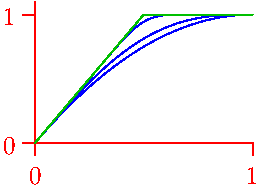
\includegraphics[scale=0.95]{bernstein}
		\end{minipage}\par\vspace{-10pt}
	  \begin{align*}
		  B_3f(x)&=f(0)(1-x)^3+3f(\tfrac 13)x(1-x)^2+3f(\tfrac 23)x^2(1-x)+f(1)x^3\\
		  &= 0(1-x)^3+ 2x(1-x)^2+3x^2(1-x)+x^3\\
		  &=x(2-x)=B_2f(x)\\[5pt]
		  B_4f(x)&=0(1-x)^4+2x(1-x)^3+ 6x^2(1-x)^2 +4x^3(1-x)+x^4\\
		  &=x(x^3-2x^2+2)
		\end{align*}
		The Bernstein polynomials $B_2f(x), B_4f(x)$ and $B_{50}f(x)$ are drawn.
		
	  
	  \item Now assume $f(x)=x$ if $x<\frac 12$ and $f(x)=1-x$ otherwise.\smallbreak
	  \begin{minipage}[t]{0.6\linewidth}\vspace{-20pt}
			\begin{gather*}
	  		B_1f(x)=f(0)(1-x)+f(1)x=0\\[5pt]
	  		B_2f(x)=x(1-x)\\[5pt]
	  		\begin{aligned}
	  			B_3f(x)&=0(1-x)^3+x(1-x)^2+x^2(1-x)+0x^3\\
	  			&=x(1-x)=B_2f(x)
				\end{aligned}
	  	\end{gather*}
		\end{minipage}
		\hfill
		\begin{minipage}[t]{0.39\linewidth}\vspace{-25pt}
			\flushright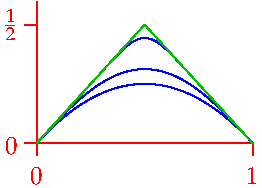
\includegraphics[scale=0.95]{bernstein2}
		\end{minipage}\par\vspace{-8pt}
	  	\begin{align*}
		  	B_4f(x)&=f(0)(1-x)^4+f(\tfrac 14)\!\cdot\! 4x(1-x)^3+f(\tfrac 12)\!\cdot\! 6x^2(1-x)^2 +f(\tfrac 34)\!\cdot\! 4x^3(1-x)+f(1)x^4\\
		  	&=x(1-x)^3+3x^2(1-x)^2 +x^3(1-x)\\
		  	&=x(1-x)(1+x-x^2)
			\end{align*}
	\end{enumerate}
\end{examples}


\clearpage


\def\ray#1{\overrightarrow{#1}}

\boldsubsubsection{Bézier curves (just for fun!)}

\begin{minipage}[t]{0.53\linewidth}\vspace{0pt}
	The Bernstein polynomials arise naturally when considering \emph{Bézier curves.} These have many applications, particularly in computer graphics. Given three points $A,B,C$, define points on the line segments $\ray{AB}$ and $\ray{BC}$ for each $t\in[0,1]$, via
	\[
		\ray{AB}(t)=(1-t)A+tB\qquad \ray{BC}(t)=(1-t)B+tC
	\]
	These points move at a constant speed along the corresponding segments. Now consider a \textcolor{blue}{point} on the \textcolor{orange}{\emph{moving} segment} between the points defined above:
\end{minipage}
\hfill
\begin{minipage}[t]{0.46\linewidth}\vspace{0pt}
	\flushright\href{http://www.math.uci.edu/~ndonalds/math140b/bezier.html}{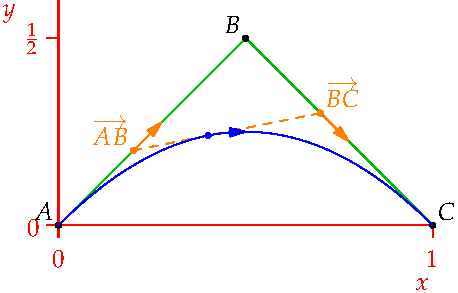
\includegraphics[scale=0.95]{bezier2}}
\end{minipage}
\smallbreak

\[
	R(t):=(1-t)\ray{AB}(t)+t\ray{BC}(t) =(1-t)^2A+2t(1-t)B+t^2C
\]
This is the \emph{quadratic Bézier curve with control points $A,B,C$.} The $2^\text{nd}$ Bernstein polynomial for a function $f$ is simply the quadratic Bézier curve with control points $\left(0,f(0)\right)$, $\left(\frac 12,f(\frac 12)\right)$ and $\left(1,f(1)\right)$. The picture\footnote{%
	Click on any of the pictures to see all of them move.%
} above shows $B_2f(x)$ for the above example.\medbreak

We can repeat the construction with more control points: with four points $A,B,C,D$, one constructs $\ray{AB}(t)$, $\ray{BC}(t)$, $\ray{CD}(t)$, then the second-order points between these, and finally the cubic Bézier curve
\begin{align*}
	R(t):&=(1-t)\left((1-t)\ray{AB}(t)+t\ray{BC}(t)\right) +t\left((1-t)\ray{BC}(t)+t\ray{CD}(t)\right)\\
	&=(1-t)^3A+3t(1-t)^2B+3t^2(1-t)C+t^3D
\end{align*}
where we now recognize the relationship to the $3^\text{rd}$ Bernstein polynomial. 
\begin{center}
	\href{http://www.math.uci.edu/~ndonalds/math140b/bezier.html}{%
		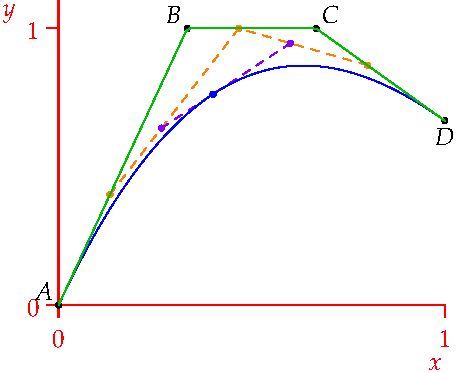
\includegraphics[scale=0.95]{bezier-cubic2}
		\qquad\quad
		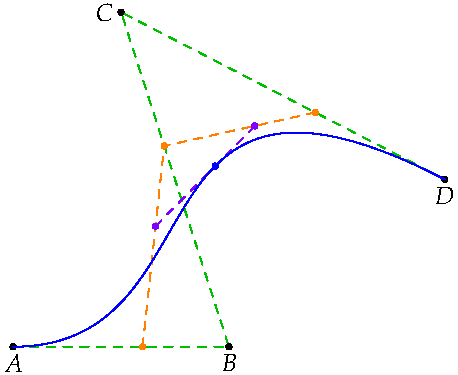
\includegraphics[scale=0.95]{bezier-cubicalt2}
	}
\end{center}
The pictures show cubic Bézier curves: the first is the graph of the Bernstein polynomial
\[
	B_3f(x)=0(1-x)^3+3x(1-x)^2+3x^2(1-x)+\tfrac 23x^3
\]
while the second is for the four given control points $A,B,C,D$.


\begin{exercises}
	\emph{Key concepts:\quad Every continuous function is the uniform limit of a polynomial sequence}


	\begin{enumerate}
	  \item Show that the closed bounded interval assumption in the approximation theorem is required by giving an example of a continuous function $f:(-1,1)\to\R$ which is \emph{not} the uniform limit of a sequence of polynomials.
	  
	  
	  \item If $g:[a,b]\to\R$ is continuous, then $f(x):=g\bigl((b-a)x+a\bigr)$ is continuous on $[0,1]$. If $P_n\to f$ uniformly on $[0,1]$, prove that $Q_n\to g$ uniformly on $[a,b]$, where
		\[
			Q_n(x)= P_n\left(\frac{x-a}{b-a}\right)
		\]
	
	
		\item Use the binomial theorem to check that every Bernstein polynomial for $f(x)=x$ is $B_nf(x)=x$ itself!
	  
	  
		\item Find a parametrization of the cubic Bézier curve with control points $(1,0)$, $(0,1)$, $(-1,0)$ and $(0,-1)$. Now sketch the curve.\par
		(\emph{Use a computer algebra package if you like!})
		
		
		\item (Hard)\lstsp Show that the Bernstein polynomials for $f(x)=x^2$ are given by 
		\[
			B_nf(x)=\frac 1nx+\frac{n-1}nx^2
		\]
		and thus verify explicitly that $B_nf\to f$ uniformly.
	\end{enumerate}
\end{exercises}

